\section{Studio della macchina a stati e relativo diagramma degli stati}
\subsection{Descrizione dello State Diagram implementato}
\begin{figure}[H]
      \centering
      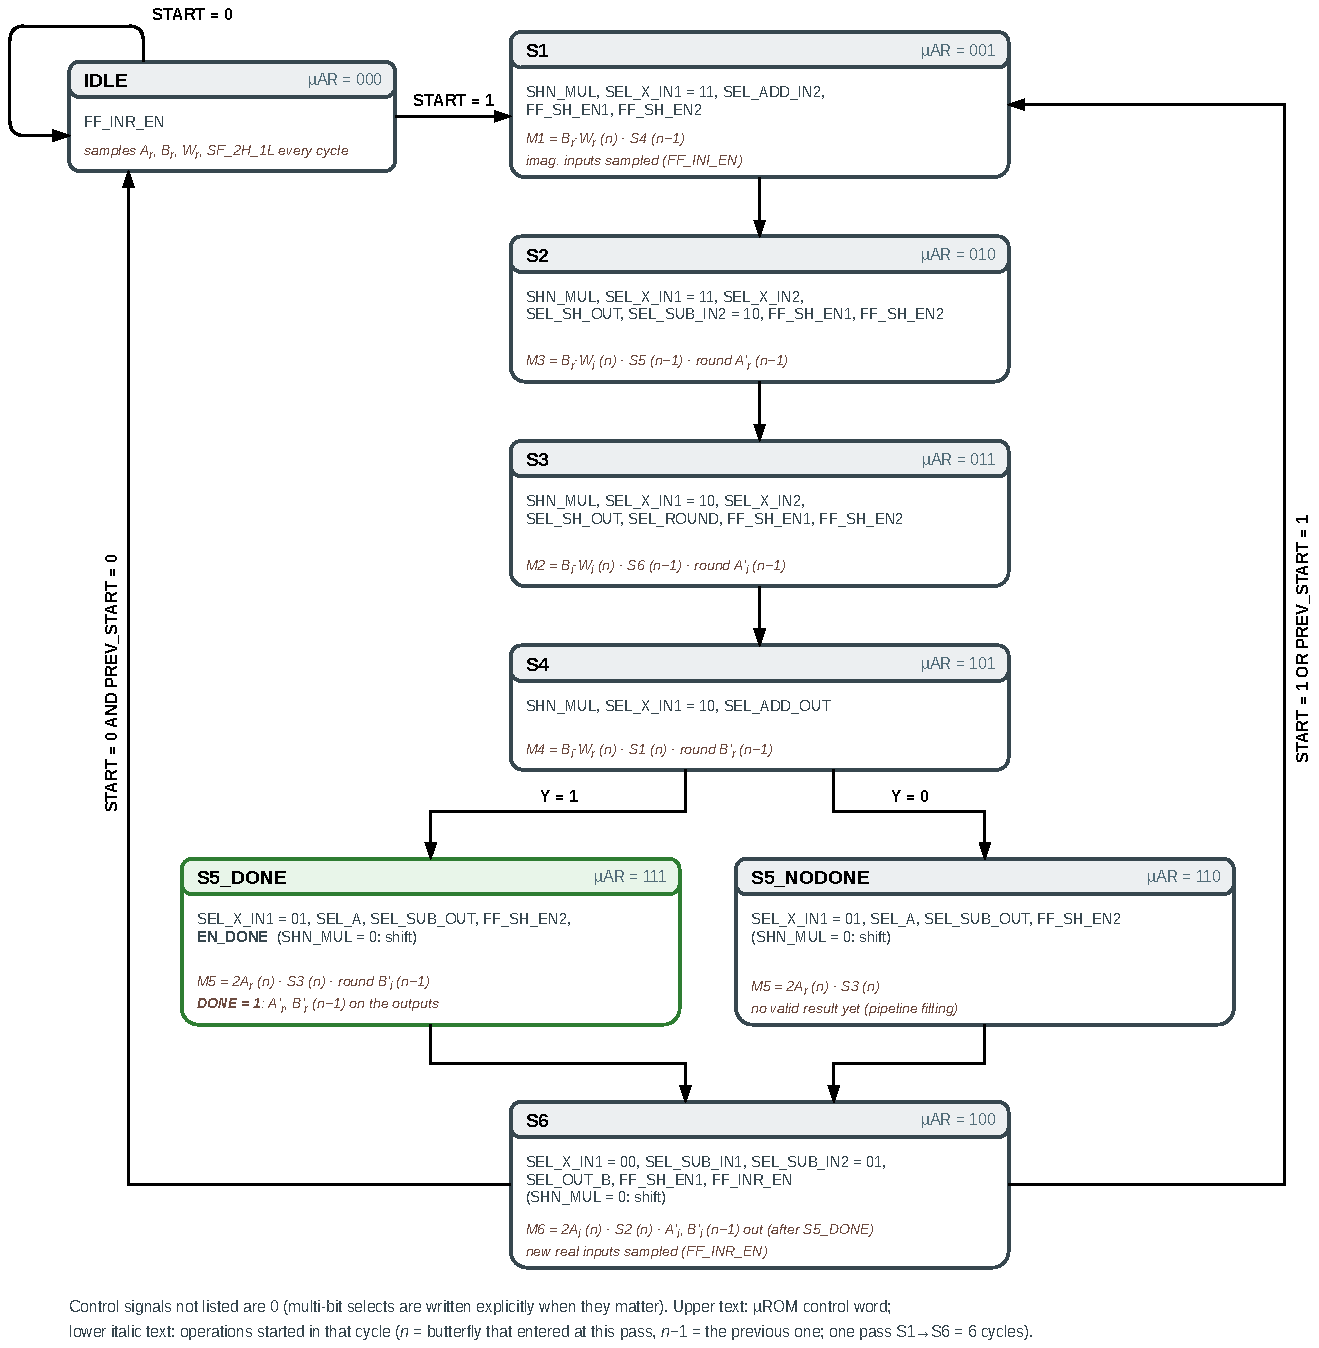
\includegraphics[width=0.93\textwidth]{fig04_state_diagram}
      \caption{Diagramma degli stati della Butterfly}
\end{figure} 
La macchina a stati sviluppata ha lo scopo di coordinare i segnali di controllo del datapath e gestire la sovrapposizione temporale delle operazioni, permettendo anche la modalità continua, come descritto in seguito nella sottosezione \ref{subsec:modalità}. In particolare, per ridurre il numero di stati utilizzati, si è scelto di ottimizzare il flusso di controllo: ciascuno stato gestisce sia l'elaborazione dei nuovi dati in ingresso, sia il completamento delle operazioni relative ai dati acquisiti al precedente segnale di $START$. Infatti, per terminare l'elaborazione degli ingressi, sono necessarie due iterazioni della sequenza di stati che vanno dallo STATO 1 allo STATO 6 (nelle figure indicati in breve come S1, \dots, S6, S5\_DONE e S5\_NODONE), senza che la macchina torni tra le due in IDLE.

\noindent Si specifica che i controlli non indicati per gli stati nello State Diagram riportato sono di default a zero; in questo, si notano 2 segnali non presenti nel datapath, che sono stati introdotti per la gestione dell'evoluzione degli stati della macchina e descritti nella sottosezione \ref{subsec:Y,PREV_START,DONE} : Y e PREV\_START. Di seguito si indica il comportamento della macchina in ciascuno degli stati presentati nel diagramma degli stati (si consiglia di leggere prima la parte relativa al ciclo attuale per ognuno degli stati, e solo alla fine leggere in ordine le descrizioni relative al ciclo precedente, per comprendere al meglio il flusso delle operazioni):
\begin{itemize}
\item Nello stato di IDLE, in cui si permane in attesa che il segnale di $START$ si abiliti, si attiva il segnale FF\_INR\_EN. Anche se la macchina è ferma, si mantiene abilitata la scrittura dei dati di input. In tal modo, si può risparmiare un ciclo di clock, poiché quando START va a uno, in corrispondenza del rising edge del clock avviene la transizione allo STATO 1 e sono già stati salvati i valori delle parti reali di $A$, $B$ e $W$. Inoltre, si campiona anche il segnale SF\_2H\_1L.

\item  Nello STATO 1, Ciclo attuale: FF\_INI\_EN è attivo e perciò le parti immaginarie di $A$, $B$ e $W$ verranno campionate al prossimo fronte di salita. SEL\_X\_IN1 =  11 instrada verso il blocco moltiplicatore $B_{r}$, mentre SEL\_X\_IN2 = 0 permette di selezionare come altro termine del prodotto $W_{r}$. Mandando ad uno il segnale SHN\_MUL, si può eseguire il prodotto $M_1 =B_{r} \cdot W_{r}$. 

\noindent Ciclo precedente: inizia la somma $S_4$ con i dati del precedente ciclo; per tale ragione, SEL\_ADD\_IN2 è impostato alto, così da indirizzare all'ingresso del sommatore $S_3$ l'ingresso voluto. Si attivano pure i segnali di enable dei due registri in cascata in uscita dallo shifter aritmetico, al fine di poter salvare il risultato di $M_6$ al prossimo fronte di salita e traslare nel secondo registro quello di $M_5$, ricavato nella precedente iterazione. Invece, SEL\_SUB\_OUT = 0, per poter salvare nel registro sottostante al sottrattore il risultato di $S_2$.

\item Nello STATO 2, Ciclo attuale:  tramite SEL\_X\_IN1 =  11, si instrada verso il blocco moltiplicatore $B_{r}$, mentre, grazie a SEL\_X\_IN2 =  1,  $W_{i}$ viene mandato all'ingresso del moltiplicatore: poiché  SHN\_MUL = 1, si effettua il prodotto $M_3 =B_{r} \cdot W_{i}$. 

\noindent Ciclo precedente: pongo  SEL\_SUB\_IN1  =  0 e SEL\_SUB\_IN2  =  10, per indirizzare i dati necessari per effettuare l'operazione di sottrazione $S_5$. In aggiunta, SEL\_ROUND = 0, per arrotondare e traslare verso destra il risultato $S_2$ (al fine di ottenere l'uscita su 24 bit $A'_r$), che verrà poi instradato verso il primo registro in uscita allo Shifter aritmetico effettuato dal blocco moltiplicatore, grazie a SEL\_SH\_OUT =  1. Poiché SEL\_ADD\_OUT =  1, il risultato dell'operazione $S_4$ verrà diretto verso il registro posto successivamente al sommatore. FF\_SH\_EN1 e FF\_SH\_EN2 sono attivi. 

 
\item  Durante lo STATO 3, Ciclo attuale:  avviene il prodotto $M_2 = B_{i} \cdot W_{i}$; infatti, viene imposto che SEL\_X\_IN1 = 10, SEL\_X\_IN2 = 1 e SHN\_MUL = 1. 

\noindent Ciclo precedente: SEL\_SH\_OUT = 1 e SEL\_ROUND = 1, al fine di arrotondare e shiftare il risultato $S_4$, per ricavare l'uscita su 24 bit $A'_i$ che viene salvata nel registro attualmente occupato da $A'_r$, il quale si sposta nel registro abilitato da FF\_SH\_EN2. Infatti, i segnali di enable FF\_SH\_EN1 e FF\_SH\_EN2 sono attivi. In questo stato viene iniziata anche l'operazione $S_6$, e termina la sottrazione $S_5$.

\item Nello STATO 4, Ciclo attuale: ci si prepara a campionare $M_3$ e si inizia il prodotto $M_4 = B_{i} \cdot W_{r}$, dato che SEL\_X\_IN1 = 10, SEL\_X\_IN2 = 0 e SHN\_MUL = 1. 
Inoltre, i controlli sono tali da fare iniziare la somma $S_1$.

\noindent Ciclo precedente:  terminano le operazioni $S_6$, si campiona $S_5$ e  poiché SEL\_ROUND = 0 e SEL\_ADD\_OUT = 1, si manda ad arrotondare $S_5$ e si ottiene il risultato su 24 bit $B'_r$, il quale è pronto per essere salvato dal registro presente all'uscita del sommatore.
Si disattivano i registri in cascata allo shifter aritmetico per non perdere i valori in essi salvati di $A'_r$ e $A'_i$.

\noindent Da questo stato è presente un salto a due vie,  dipendente dal valore della  variabile Y. Se Y = 1, i dati il cui trattamento è iniziato nell'iterazione precedente sono pronti per essere trasmessi dal prossimo colpo di clock: si passa allo STATO 5\_DONE. Invece, se Y = 0, i risultati non sono ancora pronti; si transisce, di conseguenza, allo STATO 5\_NODONE.

\item  Nello STATO 5 (sia \_DONE che \_NODONE): si ha il set degli enable per campionare, al prossimo rise, le operazioni $S_1$ e $M_2$;  viene iniziato il calcolo della somma $S_3$, dato che  SEL\_A = 1 e SEL\_ADD\_IN2 = 0. Dal momento che SEL\_X\_IN1 =  01 e SHN\_MUL = 0, si verifica lo shift di $A_{r}$ ($M_5 = 2A_{r}$).

\noindent Ciclo precedente: si manda ad arrotondare $S_6$, per ottenere l'uscita $B'_i$, pronta ad essere salvata nel registro a valle del sottrattore.

\noindent Nello STATO 5\_DONE si attiva il segnale esterno DONE, dato che EN\_DONE = 1 e Y = 1. In questo stato, la butterfly manda verso l'esterno due segnali validi su 24 bit, ovvero le parti reali dei risultati dell'elaborazione. Nello STATO 5\_NODONE, invece, EN\_DONE =  0: non viene generato alcun segnale di DONE, poiché non si hanno dati pronti. 


\item  Nello STATO 6, entrambi i cicli: il sommatore, il moltiplicatore e lo shifter aritmetico trasmettono alla loro uscita, rispettivamente, i risultati delle operazioni $S_3$, $M_4$ e $M_5$; per tale ragione, FF\_SH\_EN1 = 1, SEL\_SH\_OUT = 0 e SEL\_ADD\_OUT = 0. Inoltre, avendo SEL\_X\_IN1  = 00 e SHN\_MUL = 0, viene iniziato il calcolo dello shift aritmetico della parte immaginaria di A ($M_6$). Oltre a ciò, viene avviata la sottrazione $S_2$, poiché SEL\_SUB\_IN1 = 1 e SEL\_SUB\_IN2 = 01.
In tale stato, inoltre, si imposta FF\_INR\_EN = 1: ciò è necessario per campionare i nuovi input $A_r$, $B_r$, $W_r$ e SF\_2H\_1L, nel caso in cui la macchina funzioni in modalità continua. In aggiunta, se lo stato precedente della macchina era STATO 5\_DONE, in uscita vengono inviati i risultati $A'_i$ e $B'_i$ (grazie al fatto che SEL\_OUT\_B = 1).
Se si verifica la condizione (PREV\_START) OR (START), la macchina non finisce in IDLE al successivo colpo di clock, bensì salta direttamente allo STATO 1. Infatti, se uno dei due operandi della OR logica è alto, indica che è necessaria almeno un'altra iterazione della sequenza di stati STATO 1  -  STATO 6. In caso contrario, si ritorna nello stato di attesa. 

\end{itemize}


\subsection{Analisi di ulteriori segnali generati nella CU}
\label{subsec:Y,PREV_START,DONE}
\noindent Si analizzano ora altri segnali di estrema rilevanza che sono generati all'interno della unità di controllo della Butterfly.

\noindent Per prima cosa, si studia il segnale FF\_INI\_EN. Come già espresso nelle precedenti sottosezioni, quando FF\_INR\_EN risulta alto, si attivano i registri in ingresso all'unità, relativi alle parti reali dei dati in input e quelli legati al segnale che regola lo shift finale verso destra SF\_2H\_1L. Poiché, per il protocollo di comunicazione utilizzato per le Butterfly progettate, si vogliono campionare le parti immaginarie degli ingressi con un colpo di clock di ritardo rispetto alle parti reali, si è deciso di generare il segnale FF\_INI\_EN mediante un flip-flop con ingresso FF\_INR\_EN, con il beneficio di ridurre di uno la dimensione di ogni parola della $\mu ROM$ presente nell'unità di controllo del componente.

\begin{figure}[H]
      \centering
      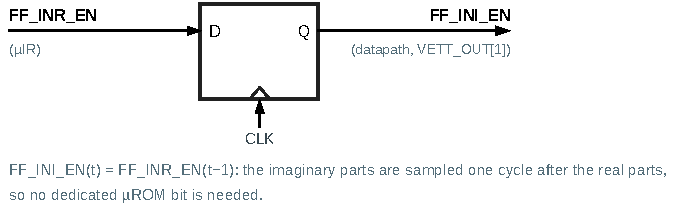
\includegraphics[width=0.7\textwidth]{fig05_ff_ini_en}
      \caption{Logica per la gestione di FF\_INI\_EN}
\end{figure} 

\noindent Invece, per gestire correttamente l'evoluzione dello stato presente della macchina, si è trovato come soluzione l'introduzione di una sorta di segnale di START ritardato. In particolare, si è aggiunto un segnale intermedio START\_INT, che di fatto è esattamente uno START ritardato di un colpo di clock, il quale è utilizzato come ingresso di un registro, che ha come segnale di enable (SEL\_ADD\_IN2) AND (SHN\_MUL). Questa scelta è dovuta al fatto che tale prodotto logico risulta pari a 1 unicamente nello STATO 1. Poiché l'architettura progettata è sensibile unicamente a un segnale di START attivo negli stati IDLE e/o 6, in tale maniera si è implementato un modo per ottenere PREV\_START, che permette di indicare alla macchina, quando si trova in STATO 6, se si era osservato uno START alto nello STATO 6 dell'iterazione precedente della sequenza di stati 1-6; infatti, in tal caso, PREV\_START=1. Nel caso in cui invece si è alla prima iterazione della sequenza di stati, allora certamente il sistema osserverà in STATO 6 che PREV\_START=1.

\begin{figure}[H]
      \centering
      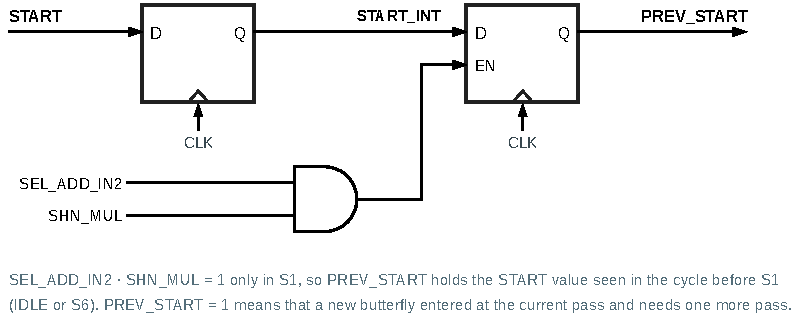
\includegraphics[width=0.85\textwidth]{fig06_prev_start}
      \caption{Descrizione del segnale PREV\_START}
\end{figure} 

\noindent Si introduce, infine, Y, un segnale utile per decidere se, quando la macchina a stati si trova nello STATO 4, deve saltare in STATO 5\_DONE per generare il segnale di fine elaborazione o meno. Se, nel quarto stato, Y risulta pari a 0, la butterfly è in fase di elaborazione, ossia i dati stanno scorrendo nei blocchi operativi del datapath, ma i risultati non sono ancora pronti; di contro, se Y = 1, il processing element è in condizione di fornire in uscita i risultati validi.

\noindent Il segnale Y coincide con l'uscita di un registro Set/Reset. Il Set è stabilito dal segnale SEL\_A, che si attiva unicamente nello STATO 5 (sia in STATO 5\_DONE che 5\_NODONE). 
\noindent La condizione di Reset, al contrario, risulta più complessa: RESET\_Y =  (FF\_INR\_EN AND $\overline{FF\_SH\_EN1}$) OR (START AND $\overline{{PREV\_START}}$ AND FF\_INR\_EN). Il primo termine della somma logica risulta alto in IDLE, così Y è già azzerato quando si attiverà un segnale di START. Inoltre, se arriva un nuovo fronte di salita di START (START = 1 e $PREV\_START$ = 0) mentre FF\_INR\_EN = 1, Y viene azzerato per preparare la nuova computazione. 

\noindent Attraverso l'uso di questo segnale così caratterizzato, si evita che dei dati assolutamente non voluti vengano validati e forniti in uscita erroneamente. 

\noindent Il segnale di DONE si ottiene invece dall'operazione logica di 'AND' tra il segnale EN\_DONE, attivo solo nello STATO 5, e Y. Di conseguenza, il DONE diventa alto solo se le parti reali dei risultati sono pronte a essere forniti in uscita.

\begin{figure}[H]
      \centering
      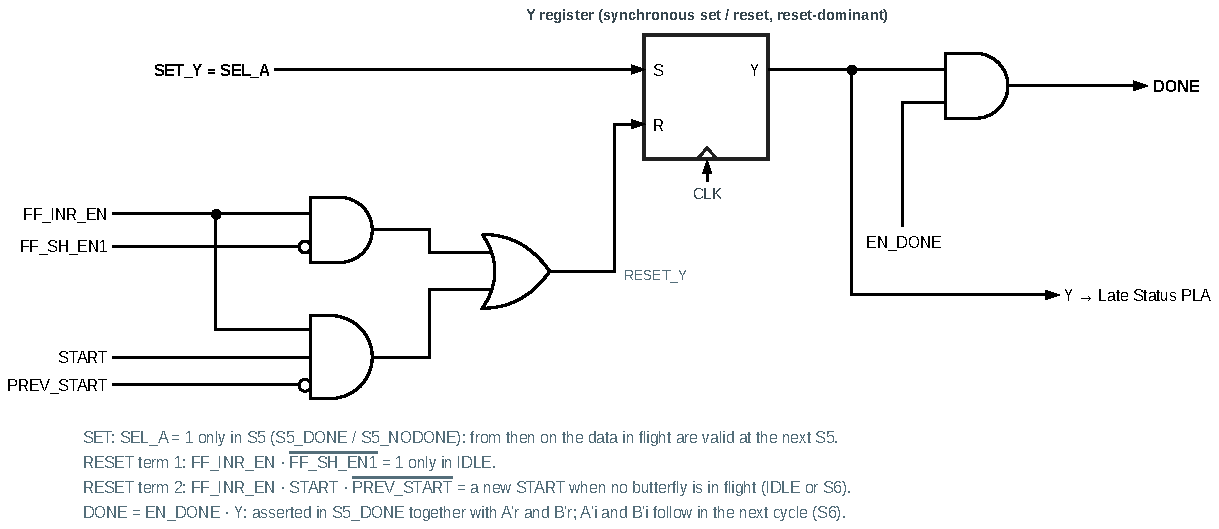
\includegraphics[width=1\textwidth]{fig07_y_done}
      \caption{Gestione  dei segnali Y e DONE}
\end{figure} 


\subsection{Modalità singola e continua}
\label{subsec:modalità}
\begin{comment}
\begin{figure}[H]
      \centering
      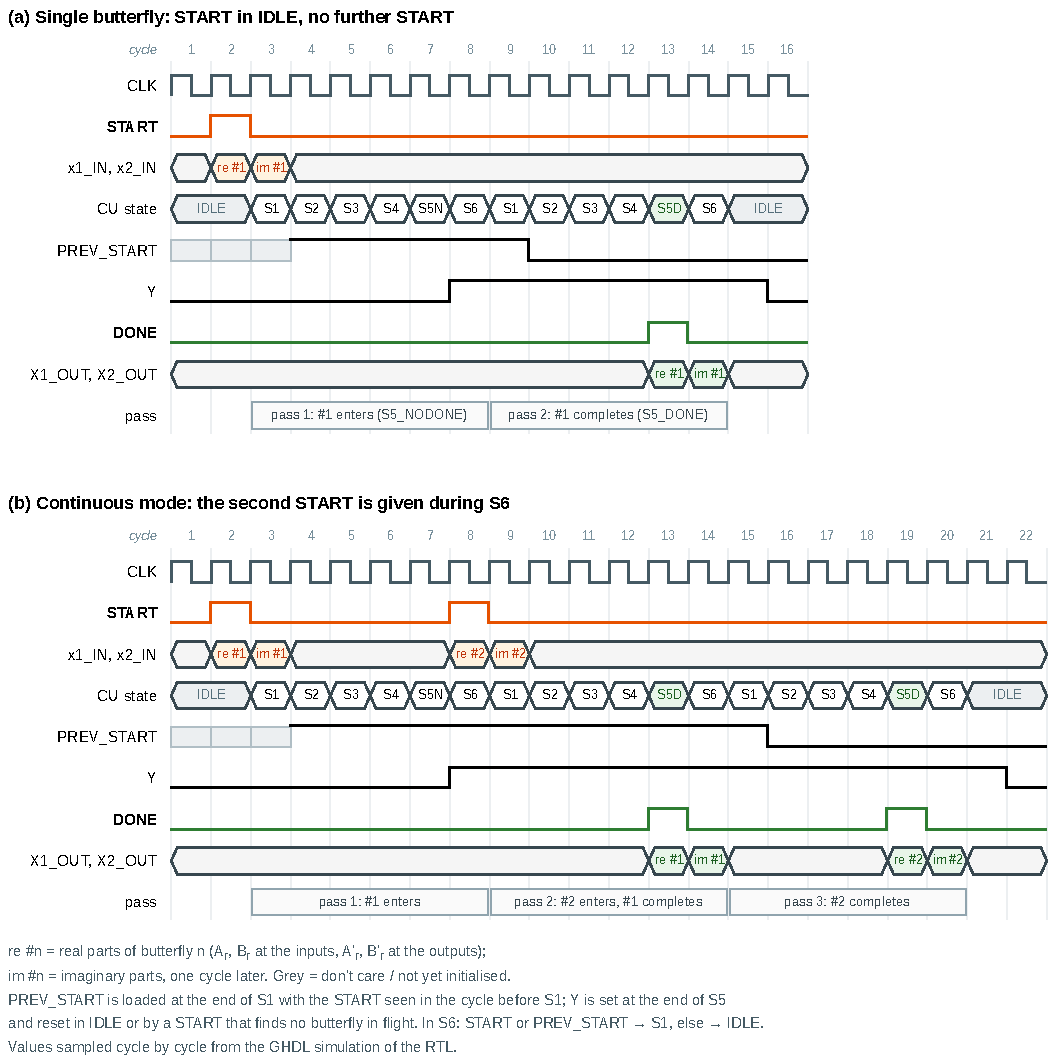
\includegraphics[width=0.7\textwidth]{fig12_single_vs_continuous}
      \caption{Rappresentazione temporale del flusso di esecuzione dei due scenari operativi di modalità continua e modalità single-shot}
\end{figure} 
\end{comment}
\noindent In questa sottosezione, si spiegano le due modalità in cui la singola butterfly (e di conseguenza tutto il sistema che permette di calcolare la FFT su 16 campioni) può lavorare.

\noindent In modalità singola, si elabora un solo pacchetto di dati per volta. Se ad esempio si parte dallo stato di IDLE, nel momento in cui arriva un nuovo START, inizia l'elaborazione dei dati in ingresso, poiché la macchina transita nello STATO 1. Quando lo stato corrente diventa lo STATO 4, si ha che $Y$ è a 0 (poiché azzerato in IDLE) e perciò la macchina passa per lo STATO 5\_NODONE, dato che si devono calcolare i nuovi valori. Dopodiché, la macchina transita in STATO 6 e Y risulta ora forzato a 1 (poiché, in STATO 5\_NODONE, SEL\_A = 1). Nel caso di modalità singola, si ha che il segnale di START in ingresso deve essere basso in questo stato. In questa istanza, si ha che, dallo STATO 6, si transita allo STATO 1, dato che, nonostante lo START disabilitato, PREV\_START vale 1. 
\noindent A questo punto, quando la macchina raggiungerà lo STATO 4, salterà in STATO 5\_DONE, fornendo in uscita le parti reali dei risultati. Al colpo di clock successivo, la macchina si trova in STATO 6 e rende disponibile in uscita le parti immaginarie ottenute dall'elaborazione. Se non si hanno altri segnali di inizio, poiché PREV\_START risulta ora pari a 0, la macchina torna in IDLE, terminando il trattamento.

\vspace{0.5cm}

\noindent La seconda modalità disponibile, quella continua, permette di aumentare il throughput dei dati in uscita. Infatti, l'idea alla base di tale modalità è che, in accordo con il Data Flow Diagram, ogni sei colpi di clock è possibile fornire dei nuovi dati di ingresso alla butterfly e iniziare la nuova elaborazione, in parallelo alla precedente che deve ancora essere completata. Ciò è permesso grazie al fatto che, dopo sei tempi di ciclo del segnale di sincronizzazione, il moltiplicatore è libero di procedere con nuove operazioni, poiché sono già state avviate le 6 moltiplicazioni richieste per l'elaborazione. Inoltre, dopo tale intervallo temporale, non sono più necessari gli ingressi precedenti, per terminare la processazione dei dati antecedenti. 

\noindent Se ad esempio si vuole entrare in modalità continua partendo dallo stato di IDLE, si procede in modo analogo al caso single-shot, con la differenza che, quando la macchina transita per la prima volta in STATO 6, si deve fornire in ingresso un valore alto del segnale di START, contemporaneamente al valore di SF\_2H\_1L e delle parti reali di $A$,$B$ e $W$. Il PE riparte dallo STATO 1, senza ritornare in IDLE, e PREV\_START rimane a 1. Inoltre, il Reset di Y non viene abilitato, permettendo il passaggio per lo STATO 5\_DONE. Attraverso questa procedura, che può essere iterata un numero arbitrario di volte, semplicemente alzando lo START quando la macchina giunge in STATO 6, è quindi possibile ricevere periodicamente dati in ingresso e produrre dei risultati validi ad ogni loop, ovvero ogni sei colpi di clock.

\noindent Quando dall'esterno lo START viene abbassato, la macchina itera ancora una volta la sequenza degli stati e finisce l'elaborazione corrente, poiché è ancora verificato che PREV\_START = 1 al momento della decisione del salto a 2 vie nello stato 6. Dal momento che Y risulta essere ancora 1, in quest'ultima iterazione si transita nuovamente in STATO 5\_DONE; nello stato successivo, poiché PREV\_START = 0, si prende la decisione di tornare nello stato di attesa, nel caso di assenza di attivazione dello START. \\

\noindent Si evidenzia che la soluzione proposta è molto versatile: infatti, grazie alla gestione del salto presente in STATO 6 e dell'implementazione dei segnali Y e PREV\_START descritti in precedenza, è possibile iniziare nuovamente un'elaborazione dati anche dallo STATO 6, senza la necessità di transire in IDLE. In questo modo, è possibile risparmiare un colpo di clock di latenza in alcune condizioni. Ad esempio, si ha la possibilità di avviare un'elaborazione singola, al termine di una processazione in modalità continua, mentre la macchina si trova ancora in STATO 6 e trasmette in uscita gli ultimi risultati $A'_i$ e $B'_i$ della modalità continua, senza necessità di tornare in IDLE. Ciò è garantito dal fatto che, nella situazione descritta, la macchina transita allo STATO 1 e Y viene resettato prima di uscire dallo stato 6, poiché FF\_INR\_EN  = 1, START = 1 e PREV\_START = 0.
